\documentclass[twoside]{book}

% Packages required by doxygen
\usepackage{fixltx2e}
\usepackage{calc}
\usepackage{doxygen}
\usepackage[export]{adjustbox} % also loads graphicx
\usepackage{graphicx}
\usepackage[utf8]{inputenc}
\usepackage{makeidx}
\usepackage{multicol}
\usepackage{multirow}
\PassOptionsToPackage{warn}{textcomp}
\usepackage{textcomp}
\usepackage[nointegrals]{wasysym}
\usepackage[table]{xcolor}

% Font selection
\usepackage[T1]{fontenc}
\usepackage[scaled=.90]{helvet}
\usepackage{courier}
\usepackage{amssymb}
\usepackage{sectsty}
\renewcommand{\familydefault}{\sfdefault}
\allsectionsfont{%
  \fontseries{bc}\selectfont%
  \color{darkgray}%
}
\renewcommand{\DoxyLabelFont}{%
  \fontseries{bc}\selectfont%
  \color{darkgray}%
}
\newcommand{\+}{\discretionary{\mbox{\scriptsize$\hookleftarrow$}}{}{}}

% Page & text layout
\usepackage{geometry}
\geometry{%
  a4paper,%
  top=2.5cm,%
  bottom=2.5cm,%
  left=2.5cm,%
  right=2.5cm%
}
\tolerance=750
\hfuzz=15pt
\hbadness=750
\setlength{\emergencystretch}{15pt}
\setlength{\parindent}{0cm}
\setlength{\parskip}{3ex plus 2ex minus 2ex}
\makeatletter
\renewcommand{\paragraph}{%
  \@startsection{paragraph}{4}{0ex}{-1.0ex}{1.0ex}{%
    \normalfont\normalsize\bfseries\SS@parafont%
  }%
}
\renewcommand{\subparagraph}{%
  \@startsection{subparagraph}{5}{0ex}{-1.0ex}{1.0ex}{%
    \normalfont\normalsize\bfseries\SS@subparafont%
  }%
}
\makeatother

% Headers & footers
\usepackage{fancyhdr}
\pagestyle{fancyplain}
\fancyhead[LE]{\fancyplain{}{\bfseries\thepage}}
\fancyhead[CE]{\fancyplain{}{}}
\fancyhead[RE]{\fancyplain{}{\bfseries\leftmark}}
\fancyhead[LO]{\fancyplain{}{\bfseries\rightmark}}
\fancyhead[CO]{\fancyplain{}{}}
\fancyhead[RO]{\fancyplain{}{\bfseries\thepage}}
\fancyfoot[LE]{\fancyplain{}{}}
\fancyfoot[CE]{\fancyplain{}{}}
\fancyfoot[RE]{\fancyplain{}{\bfseries\scriptsize Generated by Doxygen }}
\fancyfoot[LO]{\fancyplain{}{\bfseries\scriptsize Generated by Doxygen }}
\fancyfoot[CO]{\fancyplain{}{}}
\fancyfoot[RO]{\fancyplain{}{}}
\renewcommand{\footrulewidth}{0.4pt}
\renewcommand{\chaptermark}[1]{%
  \markboth{#1}{}%
}
\renewcommand{\sectionmark}[1]{%
  \markright{\thesection\ #1}%
}

% Indices & bibliography
\usepackage{natbib}
\usepackage[titles]{tocloft}
\setcounter{tocdepth}{3}
\setcounter{secnumdepth}{5}
\makeindex

% Hyperlinks (required, but should be loaded last)
\usepackage{ifpdf}
\ifpdf
  \usepackage[pdftex,pagebackref=true]{hyperref}
\else
  \usepackage[ps2pdf,pagebackref=true]{hyperref}
\fi
\hypersetup{%
  colorlinks=true,%
  linkcolor=blue,%
  citecolor=blue,%
  unicode%
}

% Custom commands
\newcommand{\clearemptydoublepage}{%
  \newpage{\pagestyle{empty}\cleardoublepage}%
}

\usepackage{caption}
\captionsetup{labelsep=space,justification=centering,font={bf},singlelinecheck=off,skip=4pt,position=top}

%===== C O N T E N T S =====

\begin{document}

% Titlepage & ToC
\hypersetup{pageanchor=false,
             bookmarksnumbered=true,
             pdfencoding=unicode
            }
\pagenumbering{alph}
\begin{titlepage}
\vspace*{7cm}
\begin{center}%
{\Large My Project }\\
\vspace*{1cm}
{\large Generated by Doxygen 1.8.13}\\
\end{center}
\end{titlepage}
\clearemptydoublepage
\pagenumbering{roman}
\tableofcontents
\clearemptydoublepage
\pagenumbering{arabic}
\hypersetup{pageanchor=true}

%--- Begin generated contents ---
\chapter{Class Index}
\section{Class List}
Here are the classes, structs, unions and interfaces with brief descriptions\+:\begin{DoxyCompactList}
\item\contentsline{section}{\hyperlink{structCOORDENADA}{C\+O\+O\+R\+D\+E\+N\+A\+DA} \\*Tipo de dados para as coordenadas }{\pageref{structCOORDENADA}}{}
\item\contentsline{section}{\hyperlink{structESTADO}{E\+S\+T\+A\+DO} \\*Tipo de dados para o estado }{\pageref{structESTADO}}{}
\item\contentsline{section}{\hyperlink{structJOGADA}{J\+O\+G\+A\+DA} \\*Tipo de dados para a jogada }{\pageref{structJOGADA}}{}
\end{DoxyCompactList}

\chapter{File Index}
\section{Lista de ficheiros}
Lista de todos os ficheiros documentados com uma breve descrição\+:\begin{DoxyCompactList}
\item\contentsline{section}{\hyperlink{camadadados_8h}{camadadados.\+h} }{\pageref{camadadados_8h}}{}
\item\contentsline{section}{\hyperlink{interface_8h}{interface.\+h} }{\pageref{interface_8h}}{}
\item\contentsline{section}{\hyperlink{lista_8h}{lista.\+h} }{\pageref{lista_8h}}{}
\item\contentsline{section}{\hyperlink{logica_8h}{logica.\+h} }{\pageref{logica_8h}}{}
\end{DoxyCompactList}

\chapter{Class Documentation}
\hypertarget{structCOORDENADA}{}\section{C\+O\+O\+R\+D\+E\+N\+A\+DA Struct Reference}
\label{structCOORDENADA}\index{C\+O\+O\+R\+D\+E\+N\+A\+DA@{C\+O\+O\+R\+D\+E\+N\+A\+DA}}
\subsection*{Public Attributes}
\begin{DoxyCompactItemize}
\item 
\mbox{\Hypertarget{structCOORDENADA_adfbc8d4856ce807139fdf62e00aed29a}\label{structCOORDENADA_adfbc8d4856ce807139fdf62e00aed29a}} 
int {\bfseries coluna}
\item 
\mbox{\Hypertarget{structCOORDENADA_aefe14bcc5a066ac3b21500cc3d28c06f}\label{structCOORDENADA_aefe14bcc5a066ac3b21500cc3d28c06f}} 
int {\bfseries linha}
\end{DoxyCompactItemize}


The documentation for this struct was generated from the following file\+:\begin{DoxyCompactItemize}
\item 
camadadados.\+h\end{DoxyCompactItemize}

\hypertarget{structESTADO}{}\section{E\+S\+T\+A\+DO Struct Reference}
\label{structESTADO}\index{E\+S\+T\+A\+DO@{E\+S\+T\+A\+DO}}


Tipo de dados para o estado.  




{\ttfamily \#include $<$Bot.\+h$>$}



Collaboration diagram for E\+S\+T\+A\+DO\+:

\hypertarget{structJOGADA}{}\section{J\+O\+G\+A\+DA Struct Reference}
\label{structJOGADA}\index{J\+O\+G\+A\+DA@{J\+O\+G\+A\+DA}}


Tipo de dados para a jogada.  




{\ttfamily \#include $<$Bot.\+h$>$}



Collaboration diagram for J\+O\+G\+A\+DA\+:
% FIG 0
\subsection*{Public Attributes}
\begin{DoxyCompactItemize}
\item 
\mbox{\Hypertarget{structJOGADA_a93d9306cb0c49b66b7d9a615bffe0149}\label{structJOGADA_a93d9306cb0c49b66b7d9a615bffe0149}} 
\hyperlink{structCOORDENADA}{C\+O\+O\+R\+D\+E\+N\+A\+DA} {\bfseries jogador1}
\item 
\mbox{\Hypertarget{structJOGADA_ab46b16dfbdc7f2af9430c8dcdac0914b}\label{structJOGADA_ab46b16dfbdc7f2af9430c8dcdac0914b}} 
\hyperlink{structCOORDENADA}{C\+O\+O\+R\+D\+E\+N\+A\+DA} {\bfseries jogador2}
\end{DoxyCompactItemize}


\subsection{Detailed Description}
Tipo de dados para a jogada. 

The documentation for this struct was generated from the following file\+:\begin{DoxyCompactItemize}
\item 
Bot.\+h\end{DoxyCompactItemize}

\hypertarget{structnodo}{}\section{nodo Struct Reference}
\label{structnodo}\index{nodo@{nodo}}


Tipo de dados para as listas ligadas.  




{\ttfamily \#include $<$Bot.\+h$>$}



Collaboration diagram for nodo\+:
% FIG 0
\subsection*{Public Attributes}
\begin{DoxyCompactItemize}
\item 
void $\ast$ \hyperlink{structnodo_ab63adcdb83ea1fdcf4fa10f3cafc4a6a}{valor}
\item 
struct \hyperlink{structnodo}{nodo} $\ast$ \hyperlink{structnodo_a086547621a7da23b916bbe26e0855308}{prox}
\end{DoxyCompactItemize}


\subsection{Detailed Description}
Tipo de dados para as listas ligadas. 

\subsection{Member Data Documentation}
\mbox{\Hypertarget{structnodo_a086547621a7da23b916bbe26e0855308}\label{structnodo_a086547621a7da23b916bbe26e0855308}} 
\index{nodo@{nodo}!prox@{prox}}
\index{prox@{prox}!nodo@{nodo}}
\subsubsection{\texorpdfstring{prox}{prox}}
{\footnotesize\ttfamily struct \hyperlink{structnodo}{nodo}$\ast$ nodo\+::prox}

apontador para o proximo nodo \mbox{\Hypertarget{structnodo_ab63adcdb83ea1fdcf4fa10f3cafc4a6a}\label{structnodo_ab63adcdb83ea1fdcf4fa10f3cafc4a6a}} 
\index{nodo@{nodo}!valor@{valor}}
\index{valor@{valor}!nodo@{nodo}}
\subsubsection{\texorpdfstring{valor}{valor}}
{\footnotesize\ttfamily void$\ast$ nodo\+::valor}

apontador para o valor do nodo 

The documentation for this struct was generated from the following file\+:\begin{DoxyCompactItemize}
\item 
Bot.\+h\end{DoxyCompactItemize}

\chapter{File Documentation}
\hypertarget{Bot_8h}{}\section{Bot.\+h File Reference}
\label{Bot_8h}\index{Bot.\+h@{Bot.\+h}}
{\ttfamily \#include $<$stdlib.\+h$>$}\newline
{\ttfamily \#include $<$stdio.\+h$>$}\newline
{\ttfamily \#include $<$string.\+h$>$}\newline
{\ttfamily \#include \char`\"{}aux.\+h\char`\"{}}\newline
Include dependency graph for Bot.\+h\+:
\nopagebreak
\begin{figure}[H]
\begin{center}
\leavevmode
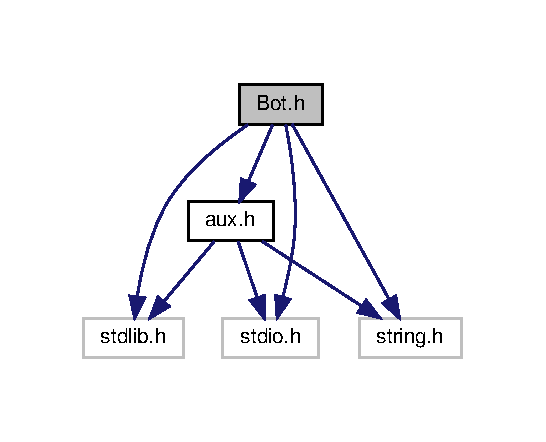
\includegraphics[width=262pt]{Bot_8h__incl}
\end{center}
\end{figure}
\subsection*{Functions}
\begin{DoxyCompactItemize}
\item 
int \hyperlink{Bot_8h_a4ed846a76c34e4a7b2ca7fc8a0176f5e}{funcao\+\_\+jogada} (\hyperlink{structESTADO}{E\+S\+T\+A\+DO} $\ast$estado)
\begin{DoxyCompactList}\small\item\em Função para efetuar uma jogada. \end{DoxyCompactList}\item 
\mbox{\Hypertarget{Bot_8h_a7e0c7e26fb685d9ab501e19b05e6954f}\label{Bot_8h_a7e0c7e26fb685d9ab501e19b05e6954f}} 
\hyperlink{structESTADO}{E\+S\+T\+A\+DO} $\ast$ \hyperlink{Bot_8h_a7e0c7e26fb685d9ab501e19b05e6954f}{inicializar\+\_\+estado} ()
\begin{DoxyCompactList}\small\item\em Inicializa um estado. \end{DoxyCompactList}\item 
\hyperlink{structCOORDENADA}{C\+O\+O\+R\+D\+E\+N\+A\+DA} \hyperlink{Bot_8h_ae89c72e4fa31dcc1eb9ba0fb8ea707e1}{get\+\_\+ultima\+\_\+jogada} (\hyperlink{structESTADO}{E\+S\+T\+A\+DO} $\ast$e)
\begin{DoxyCompactList}\small\item\em Funcao para devolver a coordenada da ultima jogada. \end{DoxyCompactList}\item 
void \hyperlink{Bot_8h_a2787d03a0237b39a69235b2a1717a34d}{altera\+\_\+estado\+\_\+casa\+\_\+preta} (\hyperlink{structESTADO}{E\+S\+T\+A\+DO} $\ast$e, \hyperlink{structCOORDENADA}{C\+O\+O\+R\+D\+E\+N\+A\+DA} c)
\begin{DoxyCompactList}\small\item\em Funcao para alterar o estado da casa para Preta. \end{DoxyCompactList}\item 
int \hyperlink{Bot_8h_ab9c95b014d2e217eae7d081088501963}{get\+\_\+jogador\+\_\+atual} (\hyperlink{structESTADO}{E\+S\+T\+A\+DO} $\ast$e)
\begin{DoxyCompactList}\small\item\em Funcao para devolver o Jogador Atual. \end{DoxyCompactList}\item 
void \hyperlink{Bot_8h_ad6e53286380cb45e6949748fe0ecf544}{floodfillaux} (\hyperlink{structESTADO}{E\+S\+T\+A\+DO} $\ast$e, int valores\mbox{[}8\mbox{]}\mbox{[}8\mbox{]}, \hyperlink{structCOORDENADA}{C\+O\+O\+R\+D\+E\+N\+A\+DA} coord, int valor)
\begin{DoxyCompactList}\small\item\em Função auxiliar para a Funcao Flood\+Fill para alterar valores do tabuleiro. \end{DoxyCompactList}\item 
\hyperlink{structCOORDENADA}{C\+O\+O\+R\+D\+E\+N\+A\+DA} \hyperlink{Bot_8h_acd6481a6f312adb939a55fb7e23a14b9}{floodfill} (\hyperlink{structESTADO}{E\+S\+T\+A\+DO} $\ast$e)
\begin{DoxyCompactList}\small\item\em Função para devolver uma Coordenada com base no algoritmo Flood\+Fill. \end{DoxyCompactList}\item 
\hyperlink{structnodo}{L\+I\+S\+TA} \hyperlink{Bot_8h_ae3b99323b6f8f35d80bb69ff1a27985e}{criar\+\_\+lista} ()
\begin{DoxyCompactList}\small\item\em Função que cria uma lista ligada. \end{DoxyCompactList}\item 
\hyperlink{structnodo}{L\+I\+S\+TA} \hyperlink{Bot_8h_a37ba5fc3cfddb6bc94d4b54b00bc696e}{insere\+\_\+cabeca} (\hyperlink{structnodo}{L\+I\+S\+TA} L, void $\ast$valor)
\begin{DoxyCompactList}\small\item\em Função que insere um nodo no ínicio da lista. \end{DoxyCompactList}\item 
\hyperlink{structnodo}{L\+I\+S\+TA} \hyperlink{Bot_8h_a4dbaee936d3b7304064647b65fced6eb}{vizinhos} (\hyperlink{structESTADO}{E\+S\+T\+A\+DO} $\ast$e, \hyperlink{structCOORDENADA}{C\+O\+O\+R\+D\+E\+N\+A\+DA} c)
\begin{DoxyCompactList}\small\item\em Função que cria uma lista com as Coordenadas dos Vizinhos de uma Coordenada. \end{DoxyCompactList}\item 
int \hyperlink{Bot_8h_ab30857ddb076ebe58da129e3e7ea7b39}{dentro\+Tabuleiro} (\hyperlink{structCOORDENADA}{C\+O\+O\+R\+D\+E\+N\+A\+DA} c)
\begin{DoxyCompactList}\small\item\em Função que testa se a Coordenada pertence ao Tabuleiro;. \end{DoxyCompactList}\item 
E\+R\+R\+OS \hyperlink{Bot_8h_a8fc889059d5c36644fbc1665d750984f}{gravar} (\hyperlink{structESTADO}{E\+S\+T\+A\+DO} $\ast$e, char $\ast$ficheiro)
\begin{DoxyCompactList}\small\item\em Grava o estado do tabuleiro. \end{DoxyCompactList}\item 
E\+R\+R\+OS \hyperlink{Bot_8h_ab752e7aff17a25212d714bd5f8c7fb12}{ler} (\hyperlink{structESTADO}{E\+S\+T\+A\+DO} $\ast$e, char $\ast$ficheiro)
\begin{DoxyCompactList}\small\item\em Função que faz a leitura do tabuleiro. \end{DoxyCompactList}\item 
int \hyperlink{Bot_8h_a7be46caf70ea549ceff7055b619e03d3}{encurralado} (\hyperlink{structESTADO}{E\+S\+T\+A\+DO} $\ast$estado, \hyperlink{structCOORDENADA}{C\+O\+O\+R\+D\+E\+N\+A\+DA} c)
\begin{DoxyCompactList}\small\item\em Verifica se uma peça está encurralada. \end{DoxyCompactList}\item 
int \hyperlink{Bot_8h_a12aba8023e2e7c4dbe26cc99c85c44fe}{verifica\+Bot\+Final} (\hyperlink{structESTADO}{E\+S\+T\+A\+DO} $\ast$e, \hyperlink{structCOORDENADA}{C\+O\+O\+R\+D\+E\+N\+A\+DA} c)
\begin{DoxyCompactList}\small\item\em Verifica se jogada leva à vitoria do jogador ou à derrota do jogador adversário. \end{DoxyCompactList}\item 
\hyperlink{structCOORDENADA}{C\+O\+O\+R\+D\+E\+N\+A\+DA} \hyperlink{Bot_8h_a5805cbe64b0343d64d0b3548d869b176}{verifica\+Check\+Mate} (\hyperlink{structESTADO}{E\+S\+T\+A\+DO} $\ast$estado)
\begin{DoxyCompactList}\small\item\em Analisa todas as jogadas possiveis fazendo uso da bot\+Final. \end{DoxyCompactList}\item 
void \hyperlink{Bot_8h_a6d1e4e9073c0dee1e5457adea4acb3e7}{inicializatab} (\hyperlink{structESTADO}{E\+S\+T\+A\+DO} $\ast$e)
\begin{DoxyCompactList}\small\item\em Funcao para inicializar um tabuleiro. \end{DoxyCompactList}\end{DoxyCompactItemize}


\subsection{Detailed Description}
Funções para utilizar listas ligadas 

\subsection{Function Documentation}
\mbox{\Hypertarget{Bot_8h_a2787d03a0237b39a69235b2a1717a34d}\label{Bot_8h_a2787d03a0237b39a69235b2a1717a34d}} 
\index{Bot.\+h@{Bot.\+h}!altera\+\_\+estado\+\_\+casa\+\_\+preta@{altera\+\_\+estado\+\_\+casa\+\_\+preta}}
\index{altera\+\_\+estado\+\_\+casa\+\_\+preta@{altera\+\_\+estado\+\_\+casa\+\_\+preta}!Bot.\+h@{Bot.\+h}}
\subsubsection{\texorpdfstring{altera\+\_\+estado\+\_\+casa\+\_\+preta()}{altera\_estado\_casa\_preta()}}
{\footnotesize\ttfamily void altera\+\_\+estado\+\_\+casa\+\_\+preta (\begin{DoxyParamCaption}\item[{\hyperlink{structESTADO}{E\+S\+T\+A\+DO} $\ast$}]{e,  }\item[{\hyperlink{structCOORDENADA}{C\+O\+O\+R\+D\+E\+N\+A\+DA}}]{c }\end{DoxyParamCaption})}



Funcao para alterar o estado da casa para Preta. 


\begin{DoxyParams}{Parameters}
{\em e} & Apontador para o estado \\
\hline
{\em c} & A coordenada a alterar \\
\hline
\end{DoxyParams}
\mbox{\Hypertarget{Bot_8h_ae3b99323b6f8f35d80bb69ff1a27985e}\label{Bot_8h_ae3b99323b6f8f35d80bb69ff1a27985e}} 
\index{Bot.\+h@{Bot.\+h}!criar\+\_\+lista@{criar\+\_\+lista}}
\index{criar\+\_\+lista@{criar\+\_\+lista}!Bot.\+h@{Bot.\+h}}
\subsubsection{\texorpdfstring{criar\+\_\+lista()}{criar\_lista()}}
{\footnotesize\ttfamily \hyperlink{structnodo}{L\+I\+S\+TA} criar\+\_\+lista (\begin{DoxyParamCaption}{ }\end{DoxyParamCaption})}



Função que cria uma lista ligada. 

\begin{DoxyReturn}{Returns}
A lista criada 
\end{DoxyReturn}
\mbox{\Hypertarget{Bot_8h_ab30857ddb076ebe58da129e3e7ea7b39}\label{Bot_8h_ab30857ddb076ebe58da129e3e7ea7b39}} 
\index{Bot.\+h@{Bot.\+h}!dentro\+Tabuleiro@{dentro\+Tabuleiro}}
\index{dentro\+Tabuleiro@{dentro\+Tabuleiro}!Bot.\+h@{Bot.\+h}}
\subsubsection{\texorpdfstring{dentro\+Tabuleiro()}{dentroTabuleiro()}}
{\footnotesize\ttfamily int dentro\+Tabuleiro (\begin{DoxyParamCaption}\item[{\hyperlink{structCOORDENADA}{C\+O\+O\+R\+D\+E\+N\+A\+DA}}]{c }\end{DoxyParamCaption})}



Função que testa se a Coordenada pertence ao Tabuleiro;. 


\begin{DoxyParams}{Parameters}
{\em c} & Coordenada \\
\hline
\end{DoxyParams}
\begin{DoxyReturn}{Returns}

\end{DoxyReturn}

\begin{DoxyParams}{Parameters}
{\em c} & Coordenada \\
\hline
\end{DoxyParams}
\begin{DoxyReturn}{Returns}
Devolve 1 se está dentro do tabuleiro 
\end{DoxyReturn}
\mbox{\Hypertarget{Bot_8h_a7be46caf70ea549ceff7055b619e03d3}\label{Bot_8h_a7be46caf70ea549ceff7055b619e03d3}} 
\index{Bot.\+h@{Bot.\+h}!encurralado@{encurralado}}
\index{encurralado@{encurralado}!Bot.\+h@{Bot.\+h}}
\subsubsection{\texorpdfstring{encurralado()}{encurralado()}}
{\footnotesize\ttfamily int encurralado (\begin{DoxyParamCaption}\item[{\hyperlink{structESTADO}{E\+S\+T\+A\+DO} $\ast$}]{estado,  }\item[{\hyperlink{structCOORDENADA}{C\+O\+O\+R\+D\+E\+N\+A\+DA}}]{c }\end{DoxyParamCaption})}



Verifica se uma peça está encurralada. 


\begin{DoxyParams}{Parameters}
{\em estado} & Apontador para o estado \\
\hline
{\em c} & Coordenada \\
\hline
\end{DoxyParams}
\mbox{\Hypertarget{Bot_8h_acd6481a6f312adb939a55fb7e23a14b9}\label{Bot_8h_acd6481a6f312adb939a55fb7e23a14b9}} 
\index{Bot.\+h@{Bot.\+h}!floodfill@{floodfill}}
\index{floodfill@{floodfill}!Bot.\+h@{Bot.\+h}}
\subsubsection{\texorpdfstring{floodfill()}{floodfill()}}
{\footnotesize\ttfamily \hyperlink{structCOORDENADA}{C\+O\+O\+R\+D\+E\+N\+A\+DA} floodfill (\begin{DoxyParamCaption}\item[{\hyperlink{structESTADO}{E\+S\+T\+A\+DO} $\ast$}]{e }\end{DoxyParamCaption})}



Função para devolver uma Coordenada com base no algoritmo Flood\+Fill. 


\begin{DoxyParams}{Parameters}
{\em e} & Apontador para o Estado \\
\hline
\end{DoxyParams}
\begin{DoxyReturn}{Returns}

\end{DoxyReturn}
\mbox{\Hypertarget{Bot_8h_ad6e53286380cb45e6949748fe0ecf544}\label{Bot_8h_ad6e53286380cb45e6949748fe0ecf544}} 
\index{Bot.\+h@{Bot.\+h}!floodfillaux@{floodfillaux}}
\index{floodfillaux@{floodfillaux}!Bot.\+h@{Bot.\+h}}
\subsubsection{\texorpdfstring{floodfillaux()}{floodfillaux()}}
{\footnotesize\ttfamily void floodfillaux (\begin{DoxyParamCaption}\item[{\hyperlink{structESTADO}{E\+S\+T\+A\+DO} $\ast$}]{e,  }\item[{int}]{valores\mbox{[}8\mbox{]}\mbox{[}8\mbox{]},  }\item[{\hyperlink{structCOORDENADA}{C\+O\+O\+R\+D\+E\+N\+A\+DA}}]{coord,  }\item[{int}]{valor }\end{DoxyParamCaption})}



Função auxiliar para a Funcao Flood\+Fill para alterar valores do tabuleiro. 


\begin{DoxyParams}{Parameters}
{\em e} & Apontador para o Estado \\
\hline
{\em valores} & Valores do Tabuleiro \\
\hline
{\em coord} & Coordenada \\
\hline
{\em valor} & Valor a implementar \\
\hline
\end{DoxyParams}
\mbox{\Hypertarget{Bot_8h_a4ed846a76c34e4a7b2ca7fc8a0176f5e}\label{Bot_8h_a4ed846a76c34e4a7b2ca7fc8a0176f5e}} 
\index{Bot.\+h@{Bot.\+h}!funcao\+\_\+jogada@{funcao\+\_\+jogada}}
\index{funcao\+\_\+jogada@{funcao\+\_\+jogada}!Bot.\+h@{Bot.\+h}}
\subsubsection{\texorpdfstring{funcao\+\_\+jogada()}{funcao\_jogada()}}
{\footnotesize\ttfamily int funcao\+\_\+jogada (\begin{DoxyParamCaption}\item[{\hyperlink{structESTADO}{E\+S\+T\+A\+DO} $\ast$}]{estado }\end{DoxyParamCaption})}



Função para efetuar uma jogada. 


\begin{DoxyParams}{Parameters}
{\em estado} & Apontador para estado; \\
\hline
{\em c} & Coordenada; \\
\hline
\end{DoxyParams}
\begin{DoxyReturn}{Returns}

\end{DoxyReturn}
\mbox{\Hypertarget{Bot_8h_ab9c95b014d2e217eae7d081088501963}\label{Bot_8h_ab9c95b014d2e217eae7d081088501963}} 
\index{Bot.\+h@{Bot.\+h}!get\+\_\+jogador\+\_\+atual@{get\+\_\+jogador\+\_\+atual}}
\index{get\+\_\+jogador\+\_\+atual@{get\+\_\+jogador\+\_\+atual}!Bot.\+h@{Bot.\+h}}
\subsubsection{\texorpdfstring{get\+\_\+jogador\+\_\+atual()}{get\_jogador\_atual()}}
{\footnotesize\ttfamily int get\+\_\+jogador\+\_\+atual (\begin{DoxyParamCaption}\item[{\hyperlink{structESTADO}{E\+S\+T\+A\+DO} $\ast$}]{e }\end{DoxyParamCaption})}



Funcao para devolver o Jogador Atual. 


\begin{DoxyParams}{Parameters}
{\em e} & Apontador para o estado\\
\hline
{\em e} & Apontador para o estado \\
\hline
\end{DoxyParams}
\begin{DoxyReturn}{Returns}
O jogador atual 
\end{DoxyReturn}
\mbox{\Hypertarget{Bot_8h_ae89c72e4fa31dcc1eb9ba0fb8ea707e1}\label{Bot_8h_ae89c72e4fa31dcc1eb9ba0fb8ea707e1}} 
\index{Bot.\+h@{Bot.\+h}!get\+\_\+ultima\+\_\+jogada@{get\+\_\+ultima\+\_\+jogada}}
\index{get\+\_\+ultima\+\_\+jogada@{get\+\_\+ultima\+\_\+jogada}!Bot.\+h@{Bot.\+h}}
\subsubsection{\texorpdfstring{get\+\_\+ultima\+\_\+jogada()}{get\_ultima\_jogada()}}
{\footnotesize\ttfamily \hyperlink{structCOORDENADA}{C\+O\+O\+R\+D\+E\+N\+A\+DA} get\+\_\+ultima\+\_\+jogada (\begin{DoxyParamCaption}\item[{\hyperlink{structESTADO}{E\+S\+T\+A\+DO} $\ast$}]{e }\end{DoxyParamCaption})}



Funcao para devolver a coordenada da ultima jogada. 


\begin{DoxyParams}{Parameters}
{\em e} & Apontador para o estado \\
\hline
\end{DoxyParams}
\begin{DoxyReturn}{Returns}
A Coordenada
\end{DoxyReturn}

\begin{DoxyParams}{Parameters}
{\em e} & Apontador para o estado \\
\hline
\end{DoxyParams}
\begin{DoxyReturn}{Returns}
A Coordenada 
\end{DoxyReturn}
\mbox{\Hypertarget{Bot_8h_a8fc889059d5c36644fbc1665d750984f}\label{Bot_8h_a8fc889059d5c36644fbc1665d750984f}} 
\index{Bot.\+h@{Bot.\+h}!gravar@{gravar}}
\index{gravar@{gravar}!Bot.\+h@{Bot.\+h}}
\subsubsection{\texorpdfstring{gravar()}{gravar()}}
{\footnotesize\ttfamily E\+R\+R\+OS gravar (\begin{DoxyParamCaption}\item[{\hyperlink{structESTADO}{E\+S\+T\+A\+DO} $\ast$}]{e,  }\item[{char $\ast$}]{ficheiro }\end{DoxyParamCaption})}



Grava o estado do tabuleiro. 


\begin{DoxyParams}{Parameters}
{\em e} & Apontador para o estado \\
\hline
{\em ficheiro} & Apontador para o nome do ficheiro \\
\hline
\end{DoxyParams}
\mbox{\Hypertarget{Bot_8h_a6d1e4e9073c0dee1e5457adea4acb3e7}\label{Bot_8h_a6d1e4e9073c0dee1e5457adea4acb3e7}} 
\index{Bot.\+h@{Bot.\+h}!inicializatab@{inicializatab}}
\index{inicializatab@{inicializatab}!Bot.\+h@{Bot.\+h}}
\subsubsection{\texorpdfstring{inicializatab()}{inicializatab()}}
{\footnotesize\ttfamily void inicializatab (\begin{DoxyParamCaption}\item[{\hyperlink{structESTADO}{E\+S\+T\+A\+DO} $\ast$}]{e }\end{DoxyParamCaption})}



Funcao para inicializar um tabuleiro. 


\begin{DoxyParams}{Parameters}
{\em e} & Apontador para o estado \\
\hline
\end{DoxyParams}
\mbox{\Hypertarget{Bot_8h_a37ba5fc3cfddb6bc94d4b54b00bc696e}\label{Bot_8h_a37ba5fc3cfddb6bc94d4b54b00bc696e}} 
\index{Bot.\+h@{Bot.\+h}!insere\+\_\+cabeca@{insere\+\_\+cabeca}}
\index{insere\+\_\+cabeca@{insere\+\_\+cabeca}!Bot.\+h@{Bot.\+h}}
\subsubsection{\texorpdfstring{insere\+\_\+cabeca()}{insere\_cabeca()}}
{\footnotesize\ttfamily \hyperlink{structnodo}{L\+I\+S\+TA} insere\+\_\+cabeca (\begin{DoxyParamCaption}\item[{\hyperlink{structnodo}{L\+I\+S\+TA}}]{L,  }\item[{void $\ast$}]{valor }\end{DoxyParamCaption})}



Função que insere um nodo no ínicio da lista. 


\begin{DoxyParams}{Parameters}
{\em l} & Lista ligada \\
\hline
{\em valor} & Apontador para o valor do nodo a inserir\\
\hline
{\em l} & Lista ligada \\
\hline
{\em valor} & Apontador para o valor do nodo a inserir \\
\hline
\end{DoxyParams}
\begin{DoxyReturn}{Returns}
A nova lista 
\end{DoxyReturn}
\mbox{\Hypertarget{Bot_8h_ab752e7aff17a25212d714bd5f8c7fb12}\label{Bot_8h_ab752e7aff17a25212d714bd5f8c7fb12}} 
\index{Bot.\+h@{Bot.\+h}!ler@{ler}}
\index{ler@{ler}!Bot.\+h@{Bot.\+h}}
\subsubsection{\texorpdfstring{ler()}{ler()}}
{\footnotesize\ttfamily E\+R\+R\+OS ler (\begin{DoxyParamCaption}\item[{\hyperlink{structESTADO}{E\+S\+T\+A\+DO} $\ast$}]{e,  }\item[{char $\ast$}]{ficheiro }\end{DoxyParamCaption})}



Função que faz a leitura do tabuleiro. 


\begin{DoxyParams}{Parameters}
{\em e} & Apontador para o estado \\
\hline
{\em ficheiro} & Apontador para o nome do ficheiro \\
\hline
\end{DoxyParams}
\mbox{\Hypertarget{Bot_8h_a12aba8023e2e7c4dbe26cc99c85c44fe}\label{Bot_8h_a12aba8023e2e7c4dbe26cc99c85c44fe}} 
\index{Bot.\+h@{Bot.\+h}!verifica\+Bot\+Final@{verifica\+Bot\+Final}}
\index{verifica\+Bot\+Final@{verifica\+Bot\+Final}!Bot.\+h@{Bot.\+h}}
\subsubsection{\texorpdfstring{verifica\+Bot\+Final()}{verificaBotFinal()}}
{\footnotesize\ttfamily int verifica\+Bot\+Final (\begin{DoxyParamCaption}\item[{\hyperlink{structESTADO}{E\+S\+T\+A\+DO} $\ast$}]{e,  }\item[{\hyperlink{structCOORDENADA}{C\+O\+O\+R\+D\+E\+N\+A\+DA}}]{c }\end{DoxyParamCaption})}



Verifica se jogada leva à vitoria do jogador ou à derrota do jogador adversário. 


\begin{DoxyParams}{Parameters}
{\em e} & Apontador para o estado \\
\hline
{\em c} & Coordenada \\
\hline
\end{DoxyParams}
\mbox{\Hypertarget{Bot_8h_a5805cbe64b0343d64d0b3548d869b176}\label{Bot_8h_a5805cbe64b0343d64d0b3548d869b176}} 
\index{Bot.\+h@{Bot.\+h}!verifica\+Check\+Mate@{verifica\+Check\+Mate}}
\index{verifica\+Check\+Mate@{verifica\+Check\+Mate}!Bot.\+h@{Bot.\+h}}
\subsubsection{\texorpdfstring{verifica\+Check\+Mate()}{verificaCheckMate()}}
{\footnotesize\ttfamily \hyperlink{structCOORDENADA}{C\+O\+O\+R\+D\+E\+N\+A\+DA} verifica\+Check\+Mate (\begin{DoxyParamCaption}\item[{\hyperlink{structESTADO}{E\+S\+T\+A\+DO} $\ast$}]{estado }\end{DoxyParamCaption})}



Analisa todas as jogadas possiveis fazendo uso da bot\+Final. 


\begin{DoxyParams}{Parameters}
{\em estado} & Apontador para o estado \\
\hline
\end{DoxyParams}
\mbox{\Hypertarget{Bot_8h_a4dbaee936d3b7304064647b65fced6eb}\label{Bot_8h_a4dbaee936d3b7304064647b65fced6eb}} 
\index{Bot.\+h@{Bot.\+h}!vizinhos@{vizinhos}}
\index{vizinhos@{vizinhos}!Bot.\+h@{Bot.\+h}}
\subsubsection{\texorpdfstring{vizinhos()}{vizinhos()}}
{\footnotesize\ttfamily \hyperlink{structnodo}{L\+I\+S\+TA} vizinhos (\begin{DoxyParamCaption}\item[{\hyperlink{structESTADO}{E\+S\+T\+A\+DO} $\ast$}]{e,  }\item[{\hyperlink{structCOORDENADA}{C\+O\+O\+R\+D\+E\+N\+A\+DA}}]{c }\end{DoxyParamCaption})}



Função que cria uma lista com as Coordenadas dos Vizinhos de uma Coordenada. 


\begin{DoxyParams}{Parameters}
{\em e} & Apontador para o Estado \\
\hline
{\em c} & Coordenada \\
\hline
\end{DoxyParams}
\begin{DoxyReturn}{Returns}
Uma Lista de Coordenadas 
\end{DoxyReturn}

%--- End generated contents ---

% Index
\backmatter
\newpage
\phantomsection
\clearemptydoublepage
\addcontentsline{toc}{chapter}{Index}
\printindex

\end{document}
